\section{Projective Geometry}
\subsection{Coordinates}
\subsubsection{Crossproduct}
$$ \bm{\tilde{x}_1} \times \bm{\tilde{x}_2} = [\bm{\tilde{x}_1}]_\times \bm{\tilde{x}_2} =
\begin{bmatrix}
0&z&-y\\
-z&0&x\\
y&-x&0\\
\end{bmatrix} \bm{\tilde{x}_2} $$
\subsubsection{2D, 3D points}
\textit{For 2D a small letter is used, a capital letter for 3D, a bold letter stands for a vector, while a normal one is a single entry from a vector}\\

\textbf{Inhomogeneous coordinates} (marked with plain letter):
$$ \bm{x} = (x,y)^\top \qquad \bm{X} = (x,y,z)^\top$$

\textbf{Homogeneous coordinates} (with a tilde on top):
$$ \tilde{\bm{x}} = (x,y,w)^\top \qquad \tilde{\bm{X}} = (x,y,z,w)^\top$$

also called " augmented coordinates $\bar{x}$ " when $w = 1$.\\

Scale is not important for incidence relation.\\

\textbf{Ideal point / point at infinity}:
$$\tilde{\bm{x}} = (x,y,0)^\top \qquad \tilde{\bm{X}} = (x,y,z,0)^\top$$

\textbf{Intersection of two lines}:
$$ \tilde{\bm{x}} = \bm{\tilde{l}_1} \times \bm{\tilde{l}_2} $$

3D Point form three planes:
$$ \begin{bmatrix}
\pi^{(1)\top}\\
\pi^{(2)\top}\\
\pi^{(3)\top}\\
\end{bmatrix} \tilde{\bm{X}} = 0 $$

\subsubsection{2D lines}

$$ \bm{l} = (a,b,c) $$

The point x lies on the line l if and only if
$$ \bm{l}^\top\tilde{\bm{x}} = ax+by+c=0$$

Line at infinity:
$$\bm{l}_\infty = (0,0,1)^\top$$

Horizontal and vertical lines:

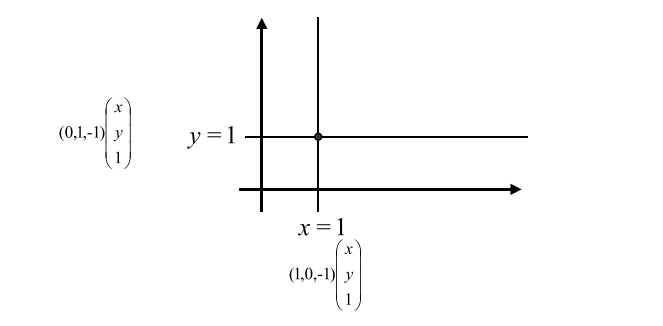
\includegraphics[width=0.8\columnwidth]{pictures/verticalhorizontal}

\textbf{Line joining two points}:
$$ \bm{l} = \bm{\tilde{x}_1} \times \bm{\tilde{x}_2} $$

\subsubsection{3D Planes}

$$ \pi = (\pi_1,\pi_2,\pi_3,\pi_4)^\top $$

The point $\bm{\tilde{X}}$ lies on the plane $\pi$ if and only if
$$ \pi^T\bm{\tilde{X}} = \pi_1x+\pi_2y+\pi_3z+\pi_4w = 0 $$

Planes from points
$$ \begin{bmatrix}
	\tilde{\bm{X}}^{(1)\top}\\
	\tilde{\bm{X}}^{(2)\top}\\
	\tilde{\bm{X}}^{(3)\top}\\
\end{bmatrix} \pi = 0 $$


\subsubsection{Conic}
Inhomogenious:
$$ ax^2 + bxy + cy^2 + dx + ey + f = 0$$

5 Degrees of freedom

\subsection{Transformation}
\subsubsection{2D Transformation}
\begin{itemize}
	\item Rotation+translation/Euclidean
	\item Scaled Rotation/Similarity/Metric - This transformation preserves angles between lines and planes( Orthogonal views of the planar at all times)
	\item Affine - Parallel lines and planes remain parallel under affine transformations (general camera motion relative to the planar shape, but always keeping sufficient distance from the planar shape)
	\item Projectivity/Collineation/Projective transformation/Homography (all cameras motions are allowed, also when moving close to the planar shape)
\end{itemize}

$$\begin{pmatrix}
x'\\
y'\\
w'\\
\end{pmatrix} = \begin{bmatrix}
h_{11}&h_{12}&h_{13}\\
h_{21}&h_{22}&h_{23}\\
h_{31}&h_{32}&h_{33}\\
\end{bmatrix} \begin{pmatrix}
x\\
y\\
w\\
\end{pmatrix} $$

Point transformation: $\bm{\tilde{x}'} = H \bm{\tilde{x}}$\\
Line transformation: $\bm{l'} = H^{-\top} \bm{l}$\\

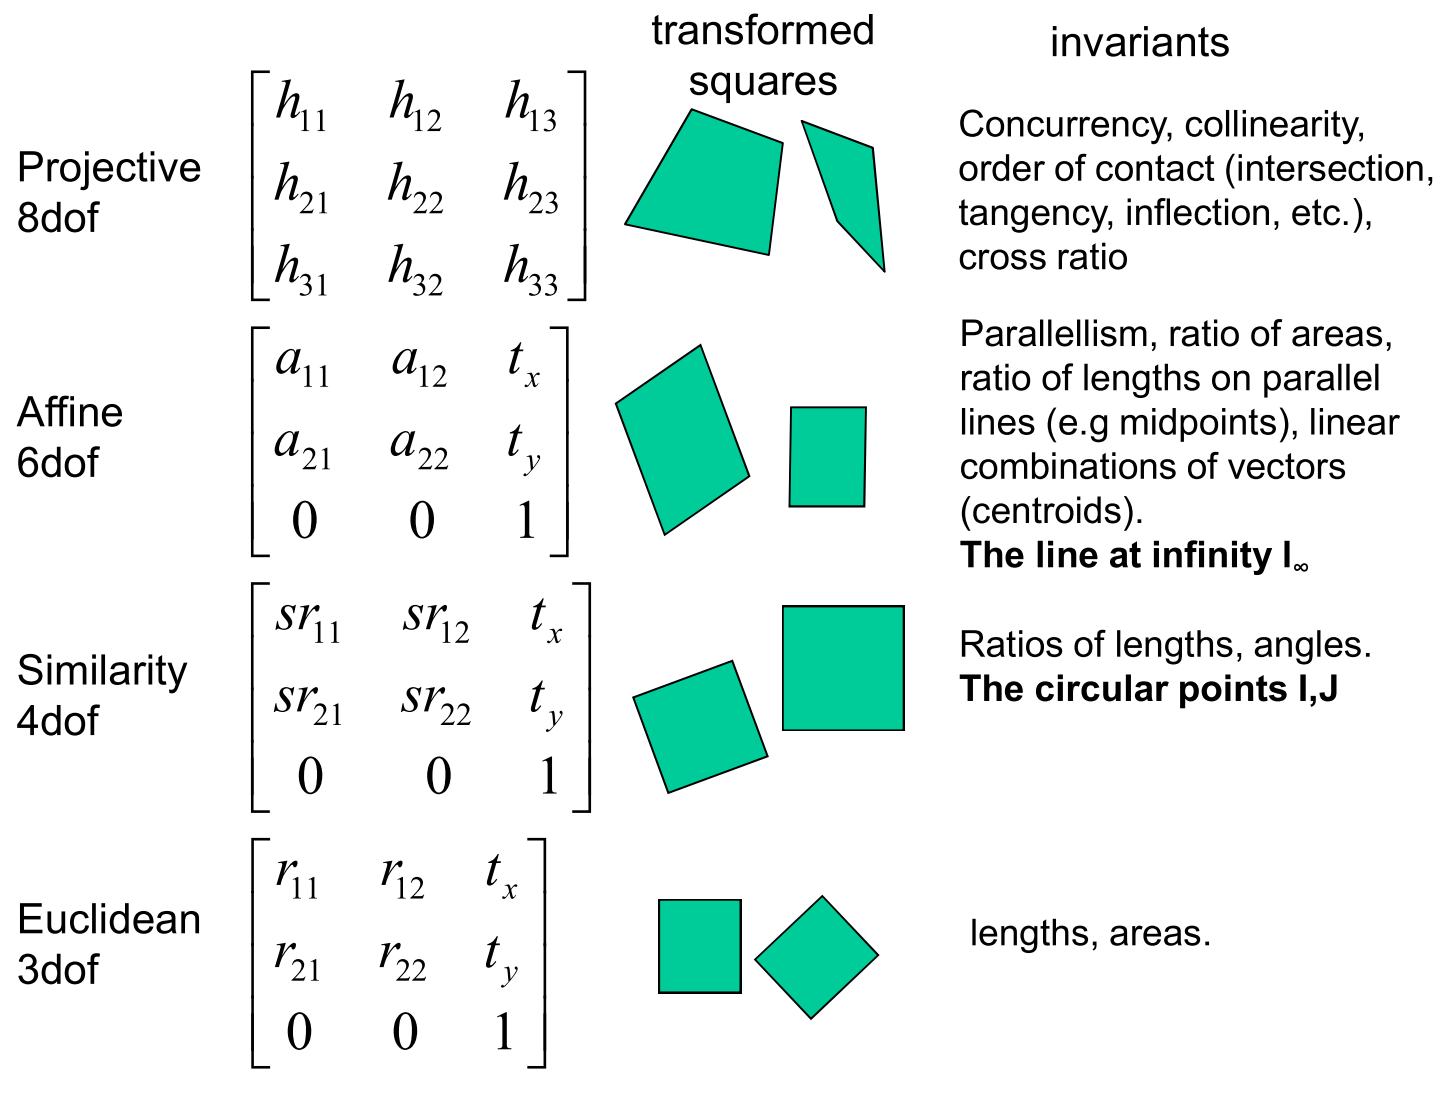
\includegraphics[width=\columnwidth]{pictures/2Dtransformations}

\subsubsection{3D Transformationen}

$$\begin{pmatrix}
x'\\
y'\\
z'\\
w'\\
\end{pmatrix} = \begin{bmatrix}
h_{11}&h_{12}&h_{13}&h_{14}\\
h_{21}&h_{22}&h_{23}&h_{24}\\
h_{31}&h_{32}&h_{33}&h_{34}\\
h_{41}&h_{42}&h_{43}&h_{44}\\
\end{bmatrix} \begin{pmatrix}
x\\
y\\
z\\
w\\
\end{pmatrix} $$

Point transformation: $\bm{\tilde{X}'} = H \bm{\tilde{X}}$\\
Plane transformation: $\bm{\pi'} = H^{-\top} \bm{\pi}$\\

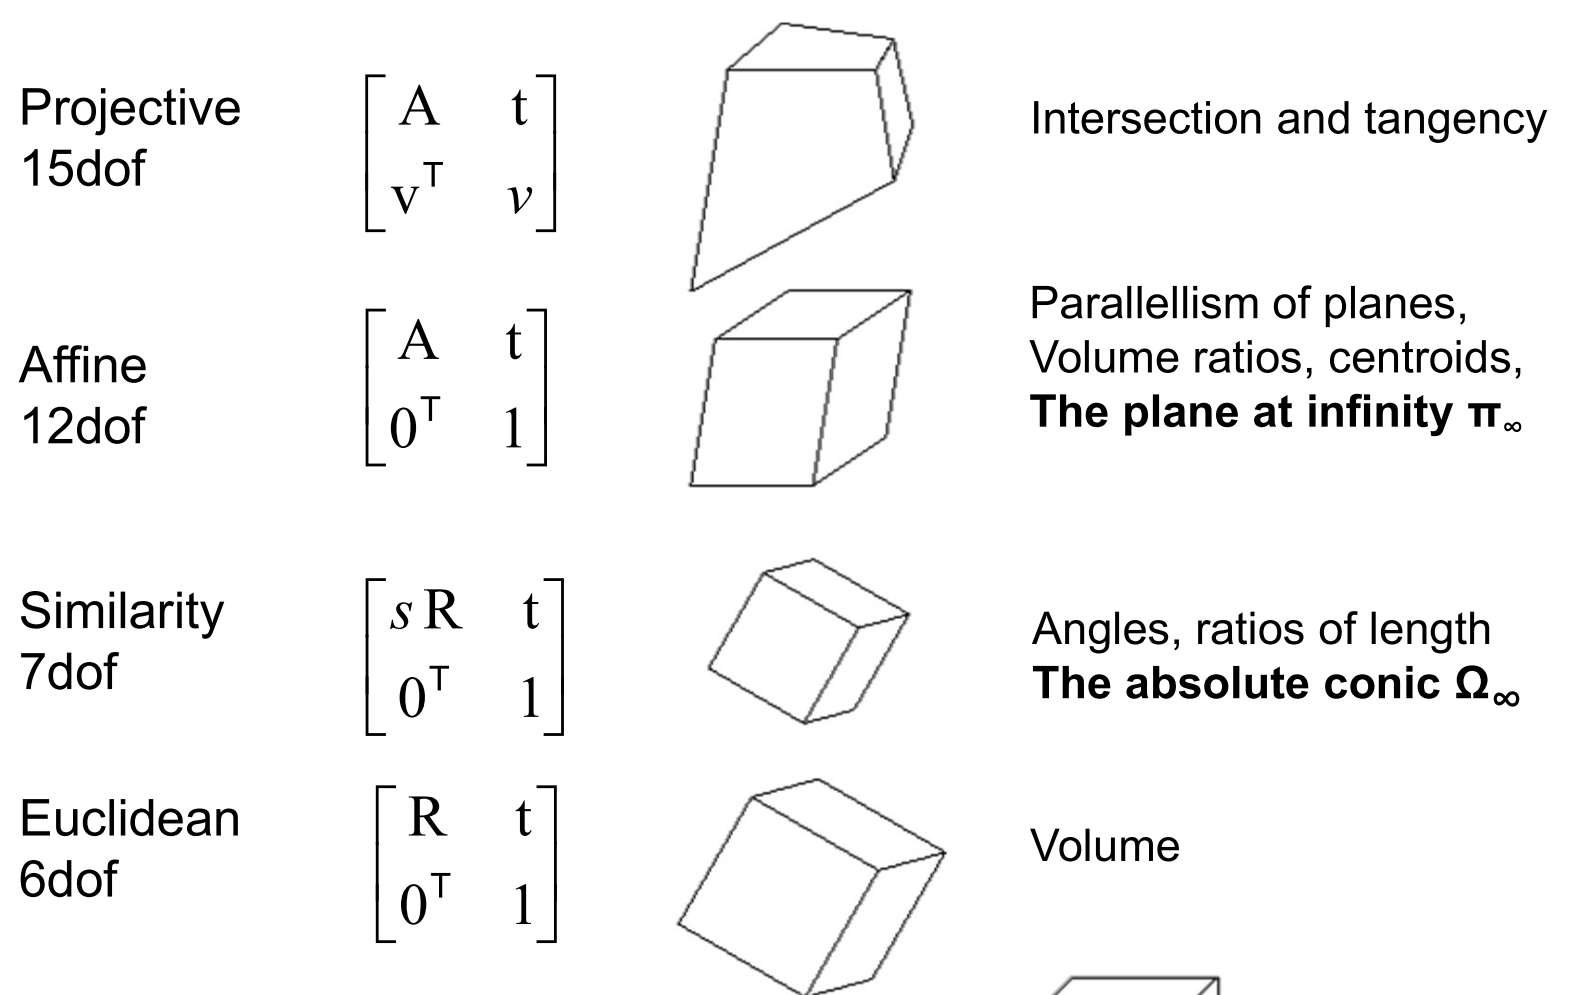
\includegraphics[width=\columnwidth]{pictures/3Dtransformation}


